%\documentclass[handout]{beamer} 
\documentclass[t,12pt,numbers,fleqn]{beamer}
%\documentclass[ignorenonframetext]{beamer}

\newif\ifquestions
%\questionstrue
\questionsfalse

\usepackage{pgfpages} 
\usepackage{hyperref}
\hypersetup{colorlinks=true,
    linkcolor=blue,
    citecolor=blue,
    filecolor=blue,
    urlcolor=blue,
    unicode=false}
\urlstyle{same}

\usepackage{booktabs}
\usepackage{bibentry}
\usepackage[round, authoryear]{natbib}
\bibliographystyle{plainnat}

%\usetheme{Iimenau}

\useoutertheme{split} %so the footline can be seen, without needing pgfpages

%\pgfpagesuselayout{resize to}[letterpaper,border shrink=5mm,landscape]  %if this is uncommented, the hyperref links do not work

\mode<presentation>{}

\input{../def-beamer}

\newcommand{\topic}{01 Introduction}

%Title page information for 1D04 lectures slides

% Define year specific parameters - used in title page and footer

\newcommand{\season}{Fall} %use to switch between Winter and Fall
\newcommand{\instructor}{Dr.~Spencer Smith} %use to switch instructor
\newcommand{\instructSmall}{Dr.~Smith}
\newcommand{\yr}{2019}
\newcommand{\courseCode}{CAS 741, CES 741}
\newcommand{\courseTitle}{Development of Scientific Computing Software}

%\setbeamerfont{structure}{series=\bfseries}
%\usefonttheme[stillsansseriftext,stillsansserifmath]{serif}
\setbeamertemplate{navigation symbols}{} 
\setbeamertemplate{itemize item}[ball]

\title{
  {\normalsize \bf 
    \borange{\courseCode~(\courseTitle)\\ \season~\yr}}\\[2ex]
  {\Large \bf \topic}}

\author[Smith]{\instructor}

\institute{
  Faculty of Engineering,
  McMaster University}

\date{
\today
%January 2011\\
\bc
  \includegraphics[scale = 0.2, keepaspectratio]
  {../mcmaster-logo-full-color.jpg}
\ec
}

\renewcommand{\borange}[1] %orange is too hard to read
{
   \bred{#1}
}

\begin{document}

\nobibliography{../../ReferenceMaterial/References}

\input{../footline}

%%%%%%%%%%%%%%%%%%%%%%%%%%%%%%%%%%%%%%%%%%%%%%%%%%%%%%

\begin{frame}
\frametitle{Introduction to CAS 741 (CES 741)}

\bi
\item Administrative details
\item Brief overview of course
\item Introductions
\item Course outline
\item Requirements
\ei
\end{frame}

%%%%%%%%%%%%%%%%%%%%%%%%%%%%%%%%%%%%%%%%%%%%%%%%%%%%%%%%%%%%%%%%%%%%%%%%%%%%%

\begin{frame}
\frametitle{Administrative Details}

\begin{itemize}

\item New Grad Stdnt Orientation: Mon, Sept 9, 10 am -- 1 pm %may
                                %cancel our class
\item Lectures: Mon and Thurs, 10:30 am -- 12:00 noon
\item Avenue for grade tracking
\begin{itemize}
\item \url{http://avenue.mcmaster.ca/} 
\item Consider putting a picture up on Avenue
\end{itemize}
\item We'll also use git on GitLab for the course material
\begin{itemize}
\item \url{https://gitlab.cas.mcmaster.ca/}
\item Create your account by logging in, option to set CAS password to MacID password
\item Course material and issue tracking at \url{https://gitlab.cas.mcmaster.ca/smiths/cas741}
\end{itemize}
\item Your projects will be hosted on GitHub
\begin{itemize}
\item \url{https://github.com/}
\item Create an account, if you do not already have one
\item Give the instructor (me) master access to your repo
\end{itemize}

\end{itemize}

\end{frame}

%%%%%%%%%%%%%%%%%%%%%%%%%%%%%%%%%%%%%%%%%%%%%%%%%%%%%%%%%%%%%%%%%%%%%%%%%%%%%

\begin{frame}
\frametitle{Overview of the Course}

\begin{itemize}

\item Application of software engineering methodologies to improve the quality
  of scientific computing software
\item \structure{What is the definition of scientific computing?}
\item \structure{What are some examples of scientific computing and scientific
    computing software?}
\item \structure{What is the definition of software engineeing?}
\item \structure{What are some techniques, tools and principles for software
    engineering?}

\end{itemize}

\end{frame}

%%%%%%%%%%%%%%%%%%%%%%%%%%%%%%%%%%%%%%%%%%%%%%%%%%%%%%%%%%%%%%%%%%%%%%%%%%%%%

\begin{frame}
\frametitle{Scientific Computing (SC)}

\begin{itemize}

\item Scientific computation consists of using computer tools to simulate
  mathematical models of real world systems so that we can better understand and
  predict the system’s behaviour.
\item Examples
\bi
\item Temperature of fuel-pin in nuclear reactor
\item Flow of pollutant in groundwater
\item Displacement of a structure
\item Thickness of cast film
\item Temperature of water in a solar water heating tank over time
\item Ordinary Differential Equation solver
\item Root finding solver etc.
\ei
\item Includes analysis, design and ``exploration'' % point made by Isobel and Alex P
\end{itemize}

\end{frame}

%%%%%%%%%%%%%%%%%%%%%%%%%%%%%%%%%%%%%%%%%%%%%%%%%%%%%%%%%%%%%%%%%%%%%%%%%%%%%

\begin{frame}
\frametitle{Software Engineering (SE)}

\begin{itemize}
\item SE is an area of engineering that deals with the development of software
  systems that
\begin{itemize}
\item Are large or complex
\item Exist in multiple versions
\item Exist for large period of time
\item Are continuously being modified
\item Are built by teams
\end{itemize}
\item SE is ``application of a systematic, disciplined, quantifiable approach to
  the development, operation and maintenance of software'' (IEEE 1990)
\item D.\ Parnas (1978) defines SE as ``multi-person
  construction of multi-version software''
\item Like other areas of engineering, SE relies heavily on
  mathematical techniques (logic and discrete math)
\item SE might be applied to SC for software certification
\end{itemize}

\end{frame}

%%%%%%%%%%%%%%%%%%%%%%%%%%%%%%%%%%%%%%%%%%%%%%%%%%%%%%%%%%%%%%%%%%%%%%%%%%%%%

\begin{frame}
\frametitle{SE Tools, Techniques and Principles}

\begin{itemize}
\item Tools
\bi
\item Programming languages
\item Version control software (git, svn, etc)
\item Debugger
\item Profiler
\item ...
\ei
\item Techniques
\bi
\item Documentation
\item Testing
\item Program families
\item Code generation
\item ...
\ei
\item Principles
\bi
\item Information hiding
\item Least privelege
\item ...
\ei
\end{itemize}

\end{frame}

%%%%%%%%%%%%%%%%%%%%%%%%%%%%%%%%%%%%%%%%%%%%%%%%%%%%%%%%%%%%%%%%%%%%%%%%%%%%%

\begin{frame}
\frametitle{Instructor}

\begin{itemize}

\item Instructor
\begin{itemize}
\item Dr.\ Spencer Smith ({\tt smiths@mcmaster.ca})
\item ITB/167
\item Drop in or make an appointment
\end{itemize}

\end{itemize}

\end{frame}

%%%%%%%%%%%%%%%%%%%%%%%%%%%%%%%%%%%%%%%%%%%%%%%%%%%%%%%%%%%%%%%%%%%%%%%%%%%%%

\begin{frame}
\frametitle{Introduction: Dr.\ Spencer Smith} 
\begin{itemize}
 
   \item Associate Professor, Department of Computing and Software.
   
   \item B.Eng.C.S, Civil Engineering Department, McMaster University. \\
         M.Eng., Ph.D., Civil Engineering Department, McMaster University.
 
   \item P.Eng.~(Licensed Professional Engineer in Ontario).
 
   \item \structure{Teaching}: Software design, scientific computing,
     introduction to computing, communication skills, software project
     management.
 
   \item \structure{Research}: Application of software engineering methodologies
     to improve the quality of scientific computing software.
 
 \end{itemize}

\end{frame}   

%%%%%%%%%%%%%%%%%%%%%%%%%%%%%%%%%%%%%%%%%%%%%%%%%%%%%%%%%%%%

\begin{frame}
\frametitle{Introductions}

\begin{itemize}
\item Your name
\item Degree program
\item Academic background
\item Experience with:
\begin{itemize}
\item Scientific computing
\item Continuous math
\item Discrete math
\item Software engineering
\item Software development technology
\bi
\item Git
\item GitHub or GitLab
\item LaTeX
\item Make etc.
\ei
\end{itemize}
\item What do you hope to get out of this course?
\end{itemize}

\end{frame}

%%%%%%%%%%%%%%%%%%%%%%%%%%%%%%%%%%%%%%%%%%%%%%%%%%%%%%%%%%%%%%%%%%%%%%%%%%%%%

\begin{frame}
\frametitle{Course Introduction}

\begin{itemize}
\item Calendar description
\begin{itemize}
\item Principles of software development for reliable and sustainable scientific
  and engineering software
\item Systematic process for development and documentation of
\bi
\item Requirements
\item System architecture
\item Detailed design
\item Implementation
\item Verification and Validation Plan
\item Verification and Validation Report
\item Code
\ei
\end{itemize}
\end{itemize}

\end{frame}

%%%%%%%%%%%%%%%%%%%%%%%%%%%%%%%%%%%%%%%%%%%%%%%%%%%%%%%%%%%%%%%%%%%%%%%%%%%%%

\begin{frame}
\frametitle{Course Project}

\begin {itemize}

\item Select a candidate SC problem
\bi
\item Requires approval from instructor
\item Will accommodate your interests as much as feasible
\item Select a project related to your research
\item Scope needs to be feasible within one term
\ei
\item Milestones
\be
\item Software Requirements Specification (SRS)
\item Module Guide (MG)
\item Module Interface Specification (MIS)
\item Implementation (and appropriate programming language)
\item VnV Plan
\item VnV Report
\ee
\item Deliverables can potentially be modified to provide project flexibility
\end {itemize}

\end{frame}

%%%%%%%%%%%%%%%%%%%%%%%%%%%%%%%%%%%%%%%%%%%%%%%%%%%%%%%%%%%%%%%%%%%%%%%%%%%%%

\begin{frame}
\frametitle{Project Selection: Desired Qualities}
\begin{itemize}
\item Related to scientific computing
\item Simple, but not trivial
\item If feasible, select a project related to your research
\item Possibly re-implement existing software
\item Each student project needs to be unique
\item Possibly a specific physical problem
\item Possibly a (family of) general purpose tool(s)
\item Some examples follow, the links are just places to get started
\end{itemize}
\end{frame}

%%%%%%%%%%%%%%%%%%%%%%%%%%%%%%%%%%%%%%%%%%%%%%%%%%

\begin{frame}

\frametitle{``Faked'' Rational Design Process}

\begin{center}
\includegraphics[scale=0.4]{../Figures/Waterfall.pdf}
\end{center}

See Parnas and Clements 1986 about ``Faking It''

\end{frame}

%%%%%%%%%%%%%%%%%%%%%%%%%%%%%%%%%%%%%%

\begin{frame}

\frametitle{Our ``Faked'' Process}

\begin{center}
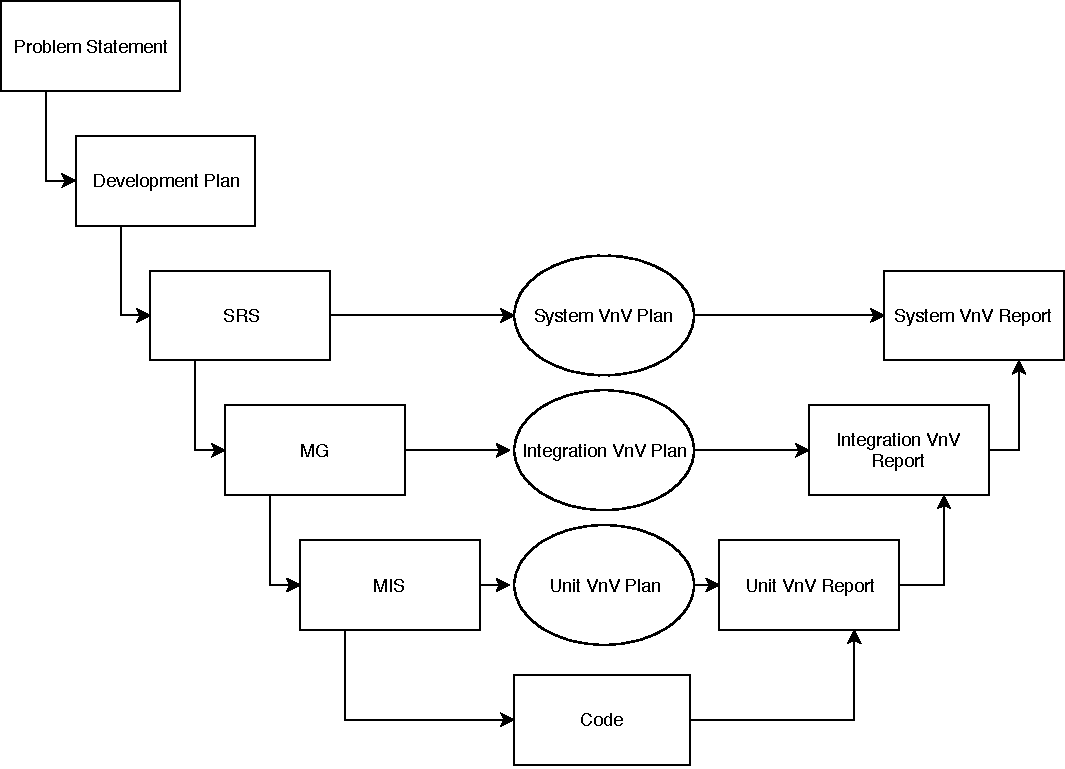
\includegraphics[scale=0.55]{../Figures/VModelOfProcess.pdf}
\end{center}
\vspace{-1.0cm}
V Model

\end{frame}

%%%%%%%%%%%%%%%%%%%%%%%%%%%%%%%%%%%%%%

\begin{frame}

\frametitle{Our Deliverables}

\begin{center}
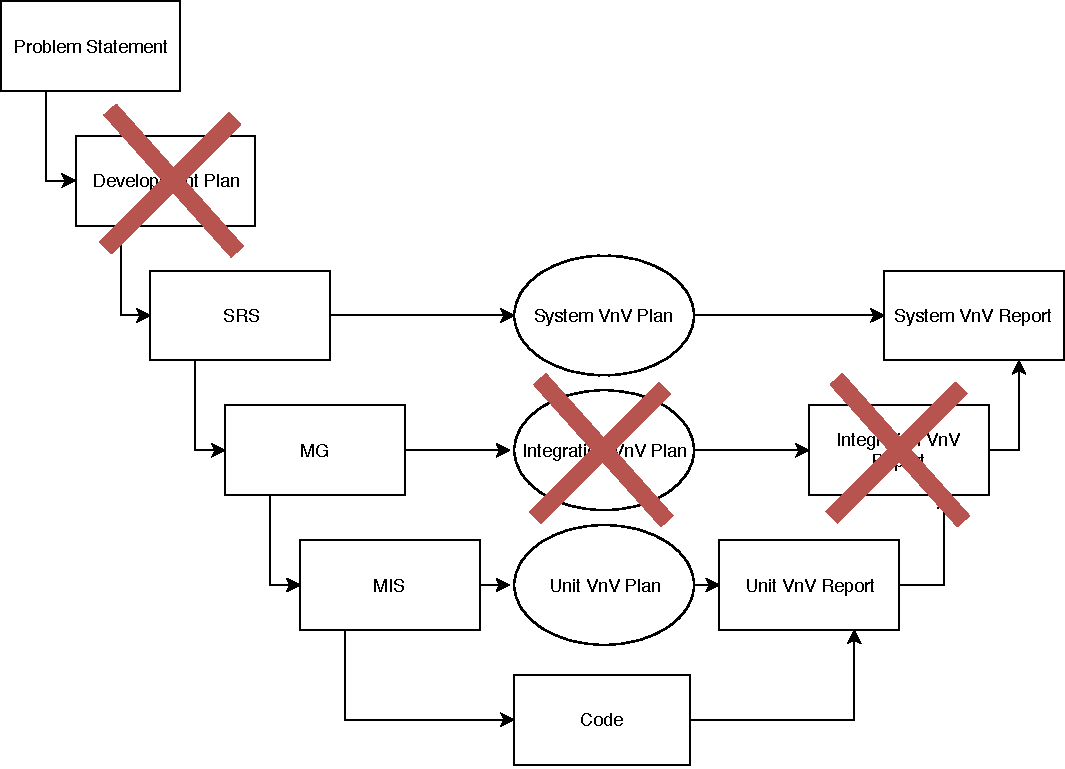
\includegraphics[scale=0.55]{../Figures/VModelOfProcessXOut.pdf}
\end{center}
\vspace{-1.0cm}
Not all docs necessary

\end{frame}

%%%%%%%%%%%%%%%%%%%%%%%%%%%%%%%%%%%%%%

\begin{frame}
\frametitle{Course Structure}

\begin {itemize}

\item Student and instructor presentations
\item Classroom discussions
\item Will present a subset of your documentation for in-class feedback
\item Structure from our documentation
\item Use GitHub issue tracker for feedback from other students

\end {itemize}

\end{frame}

%%%%%%%%%%%%%%%%%%%%%%%%%%%%%%%%%%%%%%%%%%%%%%%%%%%%%%%%%%%%%%%%%%%%%%%%%%%%%

\begin{frame}
\frametitle{Grade Assessment}

\begin {enumerate}

\item Presentations and class discussion 5\%

\item ``Domain Expert'' and secondary reviewer roles 10\%

\item Problem Statement 0\%

\item System Requirements Specification (SRS) 15\%

\item System Verification and Validation (VnV-Syst) Plan 15\%

\item Module Guide and Module Interface Specification (MG and MIS) 15\%

\item Final Documentation (including revised versions of previous documents,
  plus the source code, unit testing plan, reflection report and testing
  reports (System and Unit)) 40\%

\item Drasil simple physics example, pull request accepted 5\% (Bonus)

\end {enumerate}

\end{frame}

%%%%%%%%%%%%%%%%%%%%%%%%%%%%%%%%%%%%%%%%%%%%%%%%%%%%%%%%%%%%%%%%%%%%%%%%%%%%%

\begin{frame}
\frametitle{Policy Statements}

\begin {itemize}

\item Ideas to improve the course are welcomed
\item Missed/late work please communicate in advance, or a penalty of 20 \% per
  working day
\item If there is a problem with discrimination please contact the Department
  Chair, or other appropriate body

\end{itemize}

\end{frame}

%%%%%%%%%%%%%%%%%%%%%%%%%%%%%%%%%%%%%%%%%%%%%%%%%%%%%%%%%%%%%%%%%%%%%%%%%%%%%

\begin{frame}
\frametitle{Academic Dishonesty}

\begin {itemize}

\item Academic dishonesty consists of misrepresentation by deception or by other fraudulent means
\item Can result in serious consequences, e.g. the grade of zero on an assignment, loss of credit with a notation on
the transcript, and/or suspension or expulsion from the university.
\item It is your responsibility to understand what constitutes academic dishonesty
\item Three examples of academic dishonesty
\begin{itemize}
\item Plagiarism
\item Improper collaboration
\item Copying or using unauthorized aids in tests and examinations
\end{itemize}
\item Academic dishonesty will not be tolerated!
\end{itemize}

\end{frame}

%%%%%%%%%%%%%%%%%%%%%%%%%%%%%%%%%%%%%%%%%%%%%%%%%%%%%%%%%%%%%%%%%%%%%%%%%%%%%

\begin{frame}
\frametitle{Assigned Reading}

As often as possible, hyperlinks are included for references in the lecture
slides

\begin {itemize}

\item
  \href{https://gitlab.cas.mcmaster.ca/smiths/cas741/blob/master/ReferenceMaterial/SoftEngForScienceBook.pdf}
  {\bibentry{Smith2016}}
\item
  \href{https://gitlab.cas.mcmaster.ca/smiths/cas741/blob/master/ReferenceMaterial/SmithLaiAndKhedri2007fulltext.pdf}
  {\bibentry{SmithEtAl2007}}
\end{itemize}

\end{frame}

%%%%%%%%%%%%%%%%%%%%%%%%%%%%%%%%%%%%%%%%%%%%%%%%%%%%%%%%%%%%%%%%%%%%%%%%%%%%%

\begin{frame}
\frametitle{Assigned Reading}

\begin {itemize}

\item
  \href{https://gitlab.cas.mcmaster.ca/smiths/cas741/blob/master/ReferenceMaterial/ParnasAndClements1986.pdf}
  {\bibentry{ParnasAndClements1986}}
\item \href{https://github.com/smiths/swhs}{Solar Water Heating System Example}
\item
  \href{https://jacquescarette.github.io/Drasil/examples/SWHS/srs/SWHS_SRS.html}
  {Solar Water Heating System Example SRS (Generated by Drasil)}
\item
  \href{https://jacquescarette.github.io/Drasil/examples/Projectile/srs/Projectile_SRS.html}
  {Projectile Example SRS (Generated by Drasil)}
\item Recommended reading order for SRS documents
\begin{itemize}
\item Goal Statement
\item Instance Models
\item Requirements
\item Introduction
\item Specific System Description
\end{itemize}

\end{itemize}

\end{frame}

%%%%%%%%%%%%%%%%%%%%%%%%%%%%%%%%%%%%%%%%%%%%%%%%%%%%%%%%%%%%%%%%%%%%%%%%%%%%%

\end{document}